\chapter{Основная часть}
\section{Общие теоретические сведения}

RISC-V является открытым современным набором команд, который может использоваться для
построения как микроконтроллеров, так и высокопроизводительных микропроцессоров.
В связи с такой широкой областью применения в систему команд введена вариативность.
Таким образом, термин RISC-V фактически является названием для семейства различных систем
команд, которые строятся вокруг базового набора команд, путём внесения в него различных расширений.


В данной работе исследуется набор команд RV32I, который включает в себя основные
команды 32-битной целочисленной арифметики кроме умножения и деления. В рамках
данного набора команд мы не будем рассматривать системные команды, связанные с
таймерами, системными регистрами, управлением привилегиями, прерываниями и исключениями.

\section{Задание №1}

Варианту №20 соответствует следующая программа:

\begin{lstlisting}[label=test,caption={Программа варианта №20}]
	  .section .text
		.globl _start;
		len = 9 #Размер массива
		enroll = 2 #Количество обрабатываемых элементов за одну итерацию
		elem_sz = 4 #Размер одного элемента массива
		
		_start:
		la x1, _x
		addi x20, x0, (len-1)/enroll
		lw x31, 0(x1)
		addi x1, x1, elem_sz*1
		lp:
		lw x2, 0(x1)
		lw x3, 4(x1)
		add x1, x1, elem_sz*enroll
		bltu x2, x31, lt1
		add x31, x0, x2 #!
		lt1:    bltu x3, x31, lt2
		add x31, x0, x3
		lt2:
		addi x20, x20, -1
		bne x20, x0, lp
		lp2: j lp2
		
		.section .data
		_x:     .4byte 0x1
		.4byte 0x2
		.4byte 0x3
		.4byte 0x4
		.4byte 0x8
		.4byte 0x6
		.4byte 0x7
		.4byte 0x5
		.4byte 0x4
\end{lstlisting}

Исходя из листинга (\ref{test}) можно понять, что это программа которая ищет максимум из элементов массива, при этом обрабатывая по 2 элемента за раз.
Исходя их этого можно сказать, что в конце программы значение в регистре x31 будет равно максимальному элементу массива, то есть 8. Данной программе можно соотнести псевдокод на листинге (\ref{pseudo})

\begin{lstlisting}[label=pseudo,caption={Псевдокод программы}]
	#define len 9 \\ Размер массива
	#define enroll 2 \\ Количество элементов за итерацию
	#define elem_sz 4 \\ Размер элемента массива
	int _x[len] = {1, 2, 3, 4, 8, 6, 7, 5, 4};
	void _start() {
		int *x1 = _x;
		int x20 = x0 + (len-1)/enroll \\ В регистре x0 всегда 0;
		int x31 = x1[0];
		x1 += elem_sz;  \\ С учётом сложение адресов как char*
		do {
			int x2 = x1[0]
			int x3 = x1[elem_sz] \\ если учитывать, что адреса складываются как char*
			x1 += elem_sz * enroll;
			if !(x2 < x31) {
				x31 = x2;
			}
			if !(x3 < x31) {
				x31 = x3;
			}
			x20--;
		} while (x20 != 0);
		while(1) {};
	}
\end{lstlisting}

На листинге (\ref{disasm}) представлен дизассемблированный код с листинга (\ref{test})


\begin{lstlisting}[label=disasm,caption={Дизассемблированный код}]
	SYMBOL TABLE:
	80000000 l    d  .text	00000000 .text
	8000003c l    d  .data	00000000 .data
	00000000 l    df *ABS*	00000000 myvar.o
	00000009 l       *ABS*	00000000 len
	00000002 l       *ABS*	00000000 enroll
	00000004 l       *ABS*	00000000 elem_sz
	8000003c l       .data	00000000 _x
	80000014 l       .text	00000000 lp
	80000028 l       .text	00000000 lt1
	80000030 l       .text	00000000 lt2
	80000038 l       .text	00000000 lp2
	80000000 g       .text	00000000 _start
	80000060 g       .data	00000000 _end
	
	
	
	Disassembly of section .text:
	
	80000000 <_start>:
	80000000:	00000097          	auipc x1,0x0
	80000004:	03c08093          	addi	x1,x1,60 # 8000003c <_x>
	80000008:	00400a13          	addi	x20,x0,4
	8000000c:	0000af83          	lw	x31,0(x1)
	80000010:	00408093          	addi	x1,x1,4
	
	80000014 <lp>:
	80000014:	0000a103          	lw	x2,0(x1)
	80000018:	0040a183          	lw	x3,4(x1)
	8000001c:	00808093          	addi	x1,x1,8
	80000020:	01f16463          	bltu	x2,x31,80000028 <lt1>
	80000024:	00200fb3          	add	x31,x0,x2
	
	80000028 <lt1>:
	80000028:	01f1e463          	bltu	x3,x31,80000030 <lt2>
	8000002c:	00300fb3          	add	x31,x0,x3
	
	80000030 <lt2>:
	80000030:	fffa0a13          	addi	x20,x20,-1
	80000034:	fe0a10e3          	bne	x20,x0,80000014 <lp>
	
	80000038 <lp2>:
	80000038:	0000006f          	jal	x0,80000038 <lp2>
	
	Disassembly of section .data:
	
	8000003c <_x>:
	8000003c:	0001                	.insn	2, 0x0001
	8000003e:	0000                	.insn	2, 0x
	80000040:	0002                	.insn	2, 0x0002
	80000042:	0000                	.insn	2, 0x
	80000044:	00000003          	lb	x0,0(x0) # 0 <enroll-0x2>
	80000048:	0004                	.insn	2, 0x0004
	8000004a:	0000                	.insn	2, 0x
	8000004c:	0008                	.insn	2, 0x0008
	8000004e:	0000                	.insn	2, 0x
	80000050:	0006                	.insn	2, 0x0006
	80000052:	0000                	.insn	2, 0x
	80000054:	00000007          	.insn	4, 0x0007
	80000058:	0005                	.insn	2, 0x0005
	8000005a:	0000                	.insn	2, 0x
	8000005c:	0004                	.insn	2, 0x0004
\end{lstlisting}

\clearpage

\section{Задание №2}

Для варианта №20 требуется проследить стадии выборки и диспетчеризации для команды по адресу 8000002c, при этом 2-й итерации.
Эти стадии представлены на рисунке (\ref{fig:fetch})

\begin{figure}[h]
	\centering
	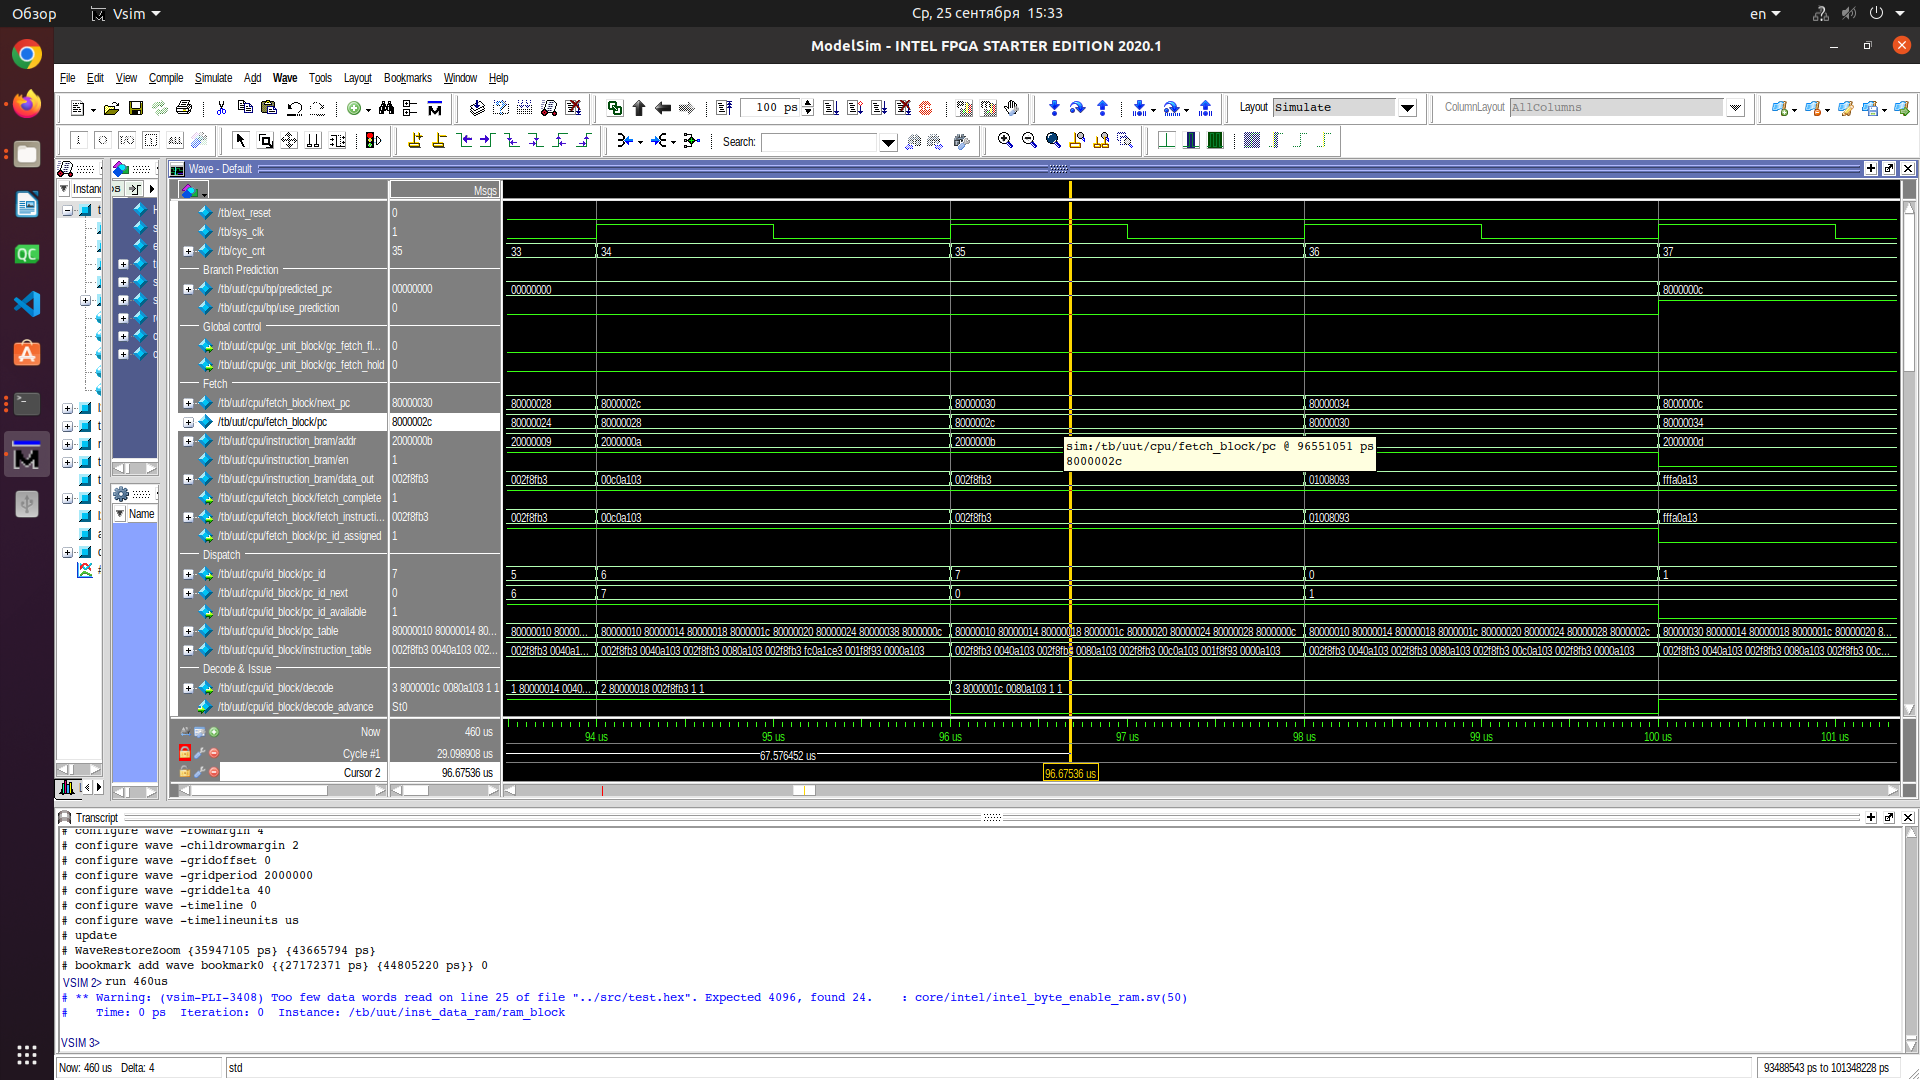
\includegraphics[width=0.9\textwidth]{fetch}
	\caption{Стадии выборки и диспетчеризации для 2-й итерации 8000002c}
	\label{fig:fetch}
\end{figure}

\clearpage

\section{Задание №3}

Для варианта №20 требуется проследить стадии декодирования и планирования для команды по адресу 80000038, при этом 2-й итерации.
Эти стадии представлены на рисунках (\ref{fig:decode}) и (\ref{fig:decode2}), так как стадии выполнялись с задержкой в такт.

\begin{figure}[h]
	\centering
	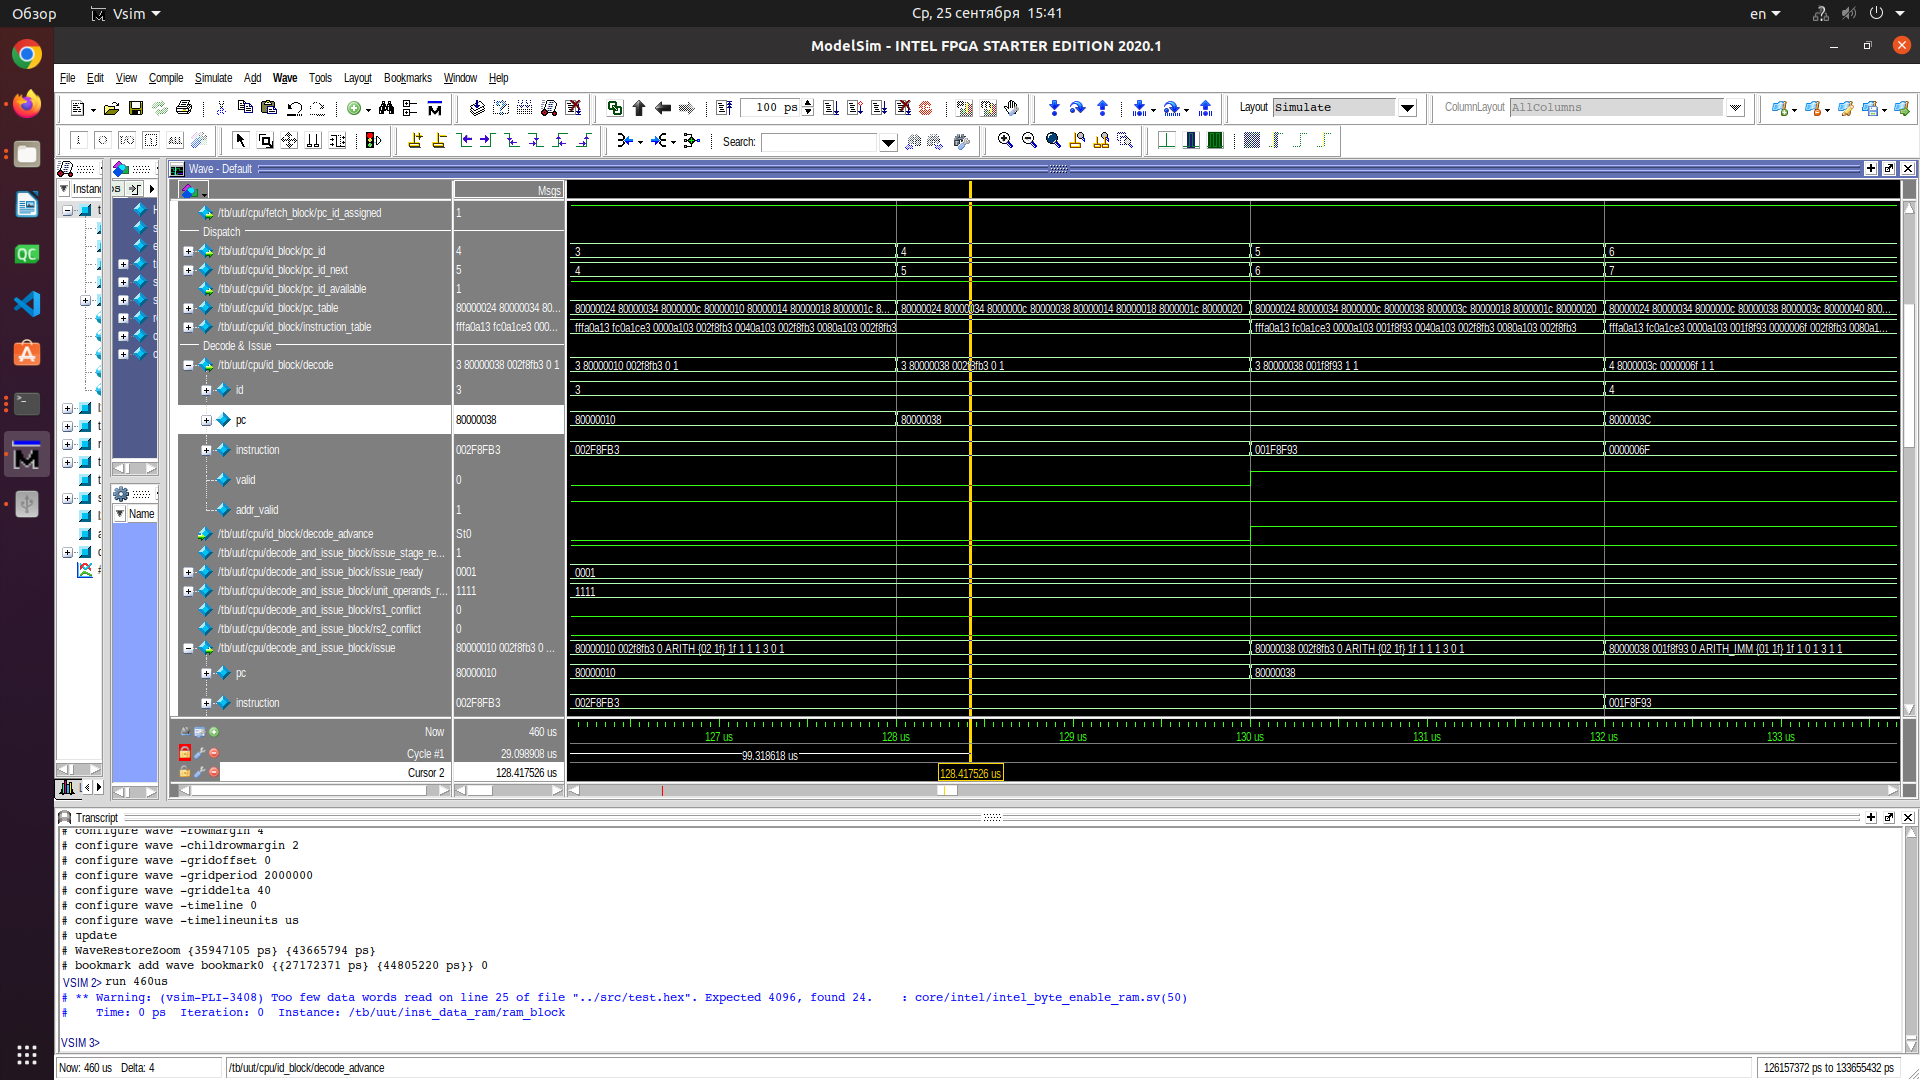
\includegraphics[width=0.9\textwidth]{decode}
	\caption{1-й такт стадии декодирования и планирования для 2-й итерации 80000038}
	\label{fig:decode}
\end{figure}


\begin{figure}[h]
	\centering
	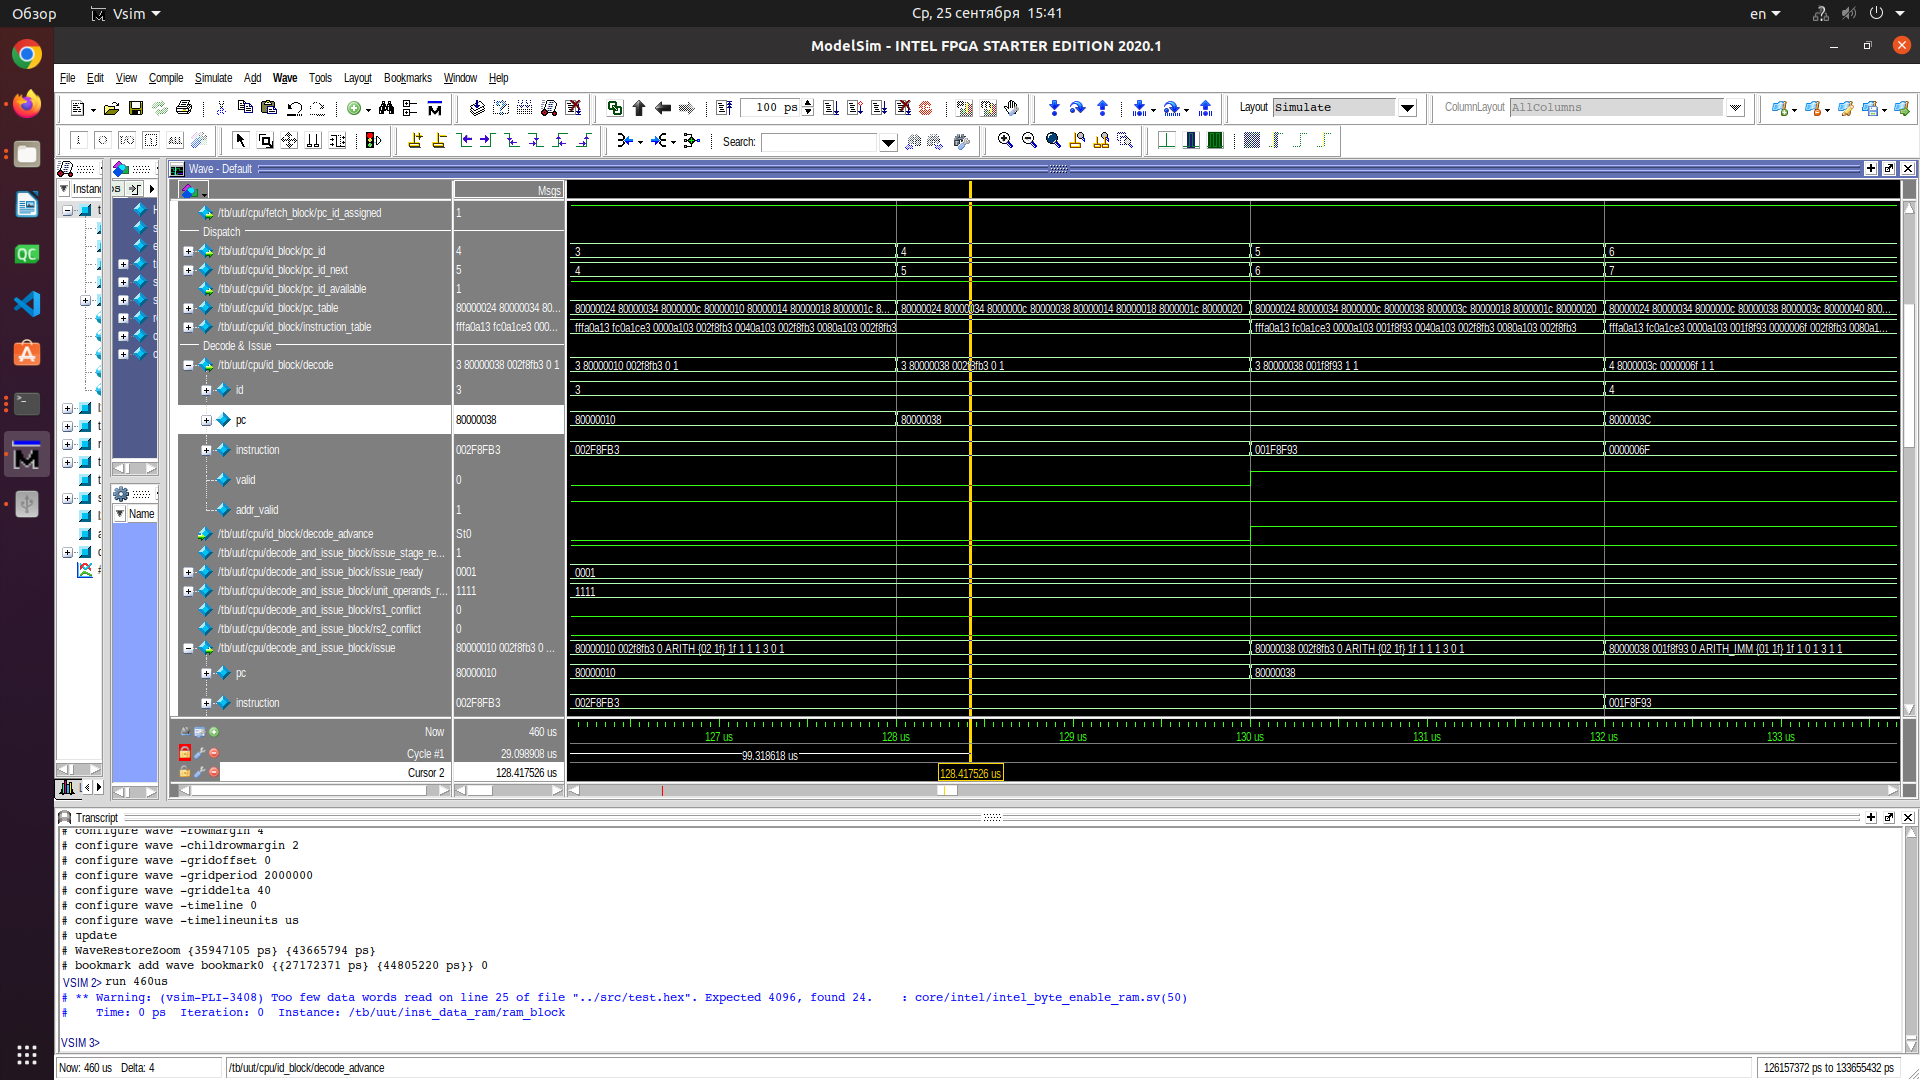
\includegraphics[width=0.9\textwidth]{decode}
	\caption{1-й такт стадии декодирования и планирования для 2-й итерации 80000038}
	\label{fig:decode2}
\end{figure}

\clearpage

\section{Задание №4}
Для варианта №20 требуется проследить стадию выполнения для команды по адресу 80000024, при этом 2-й итерации.

На рисунке (\ref{fig:decoderun}) представлена стадия декодирования,  из которой видно, что это команда имеет id=5, это команда загрузки, значит дальше команда поступит в блок LSU, а также, что команда загрузки будет идти в 3 такта.

На рисунках (\ref{fig:runstart}) и (\ref{fig:runend}) представлены 1-й и 3-й такты выполнения. На последнем видно, что команда загрузки 
с id=5 закончила выполнения.

\begin{figure}[h]
	\centering
	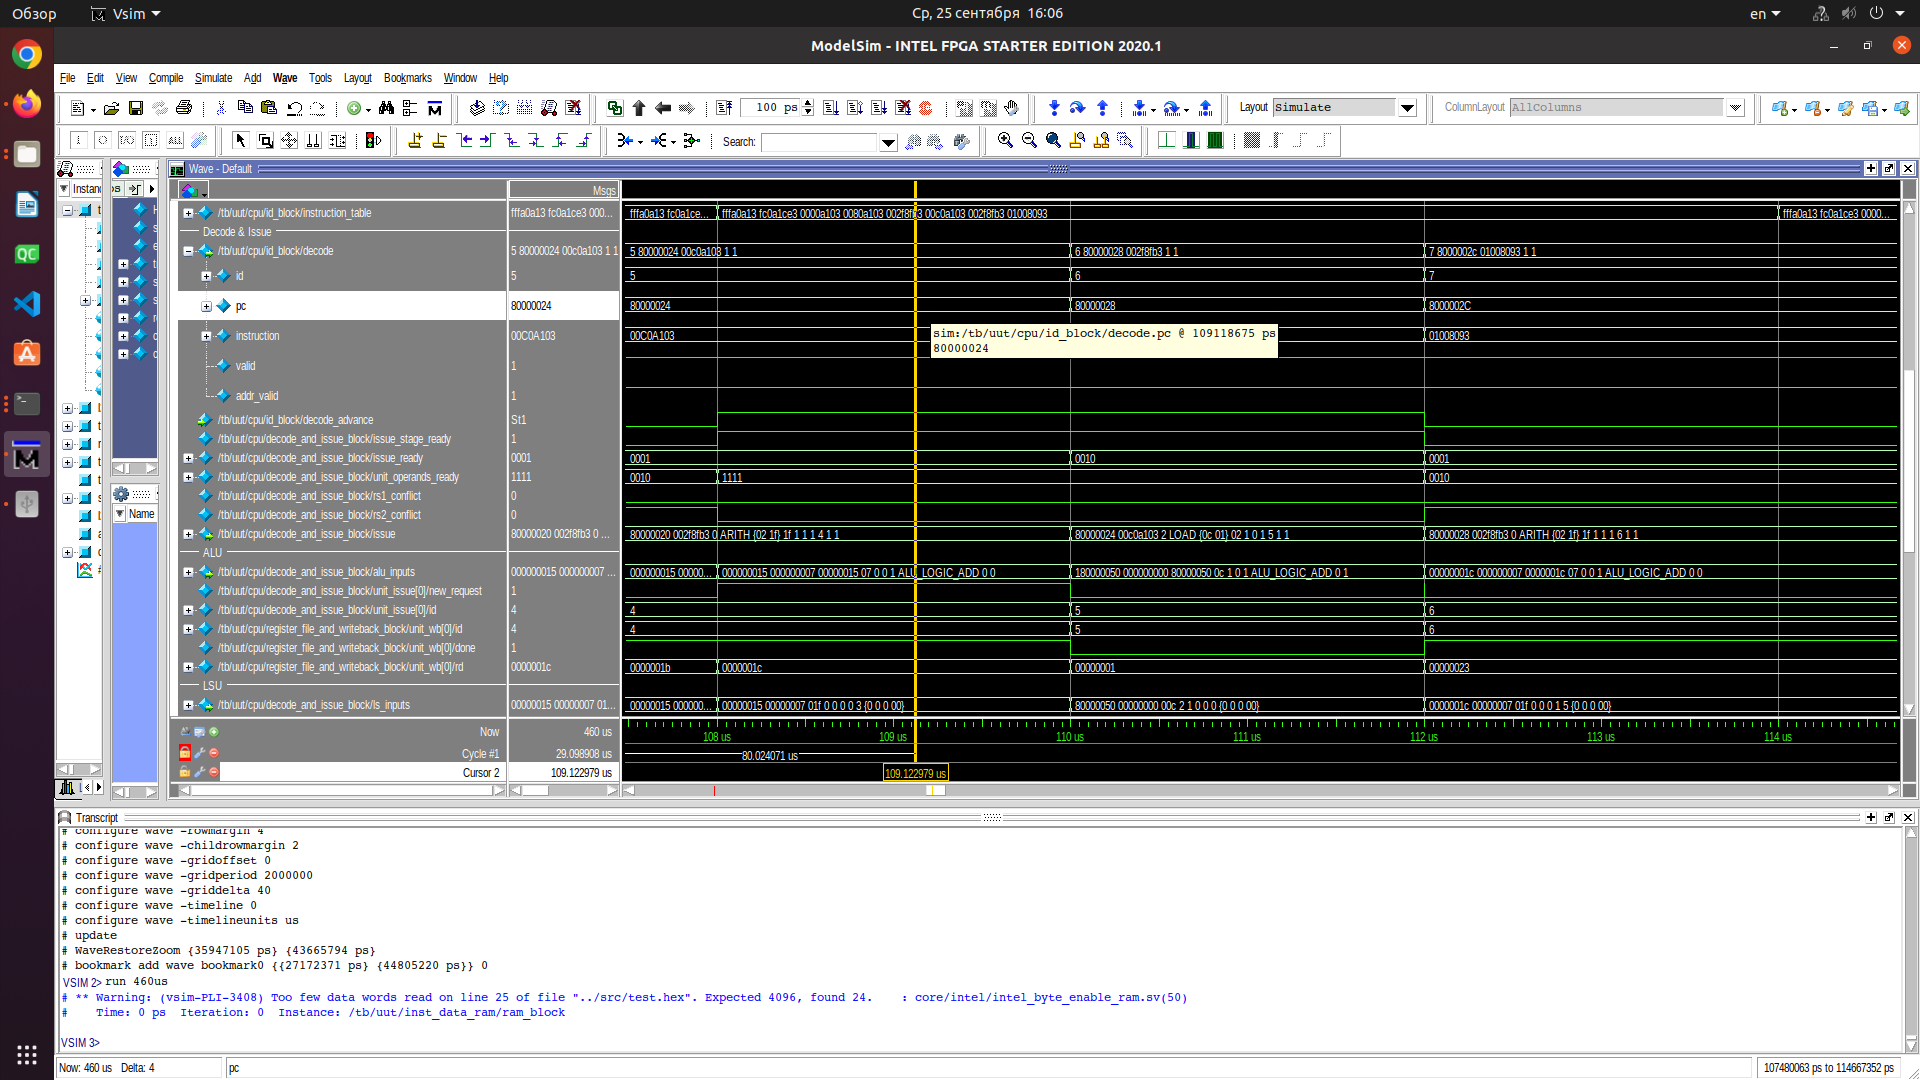
\includegraphics[width=0.9\textwidth]{decoderun}
	\caption{Стадия декодирования для 2-й итерации 80000024}
	\label{fig:decoderun}
\end{figure}

\begin{figure}[h]
	\centering
	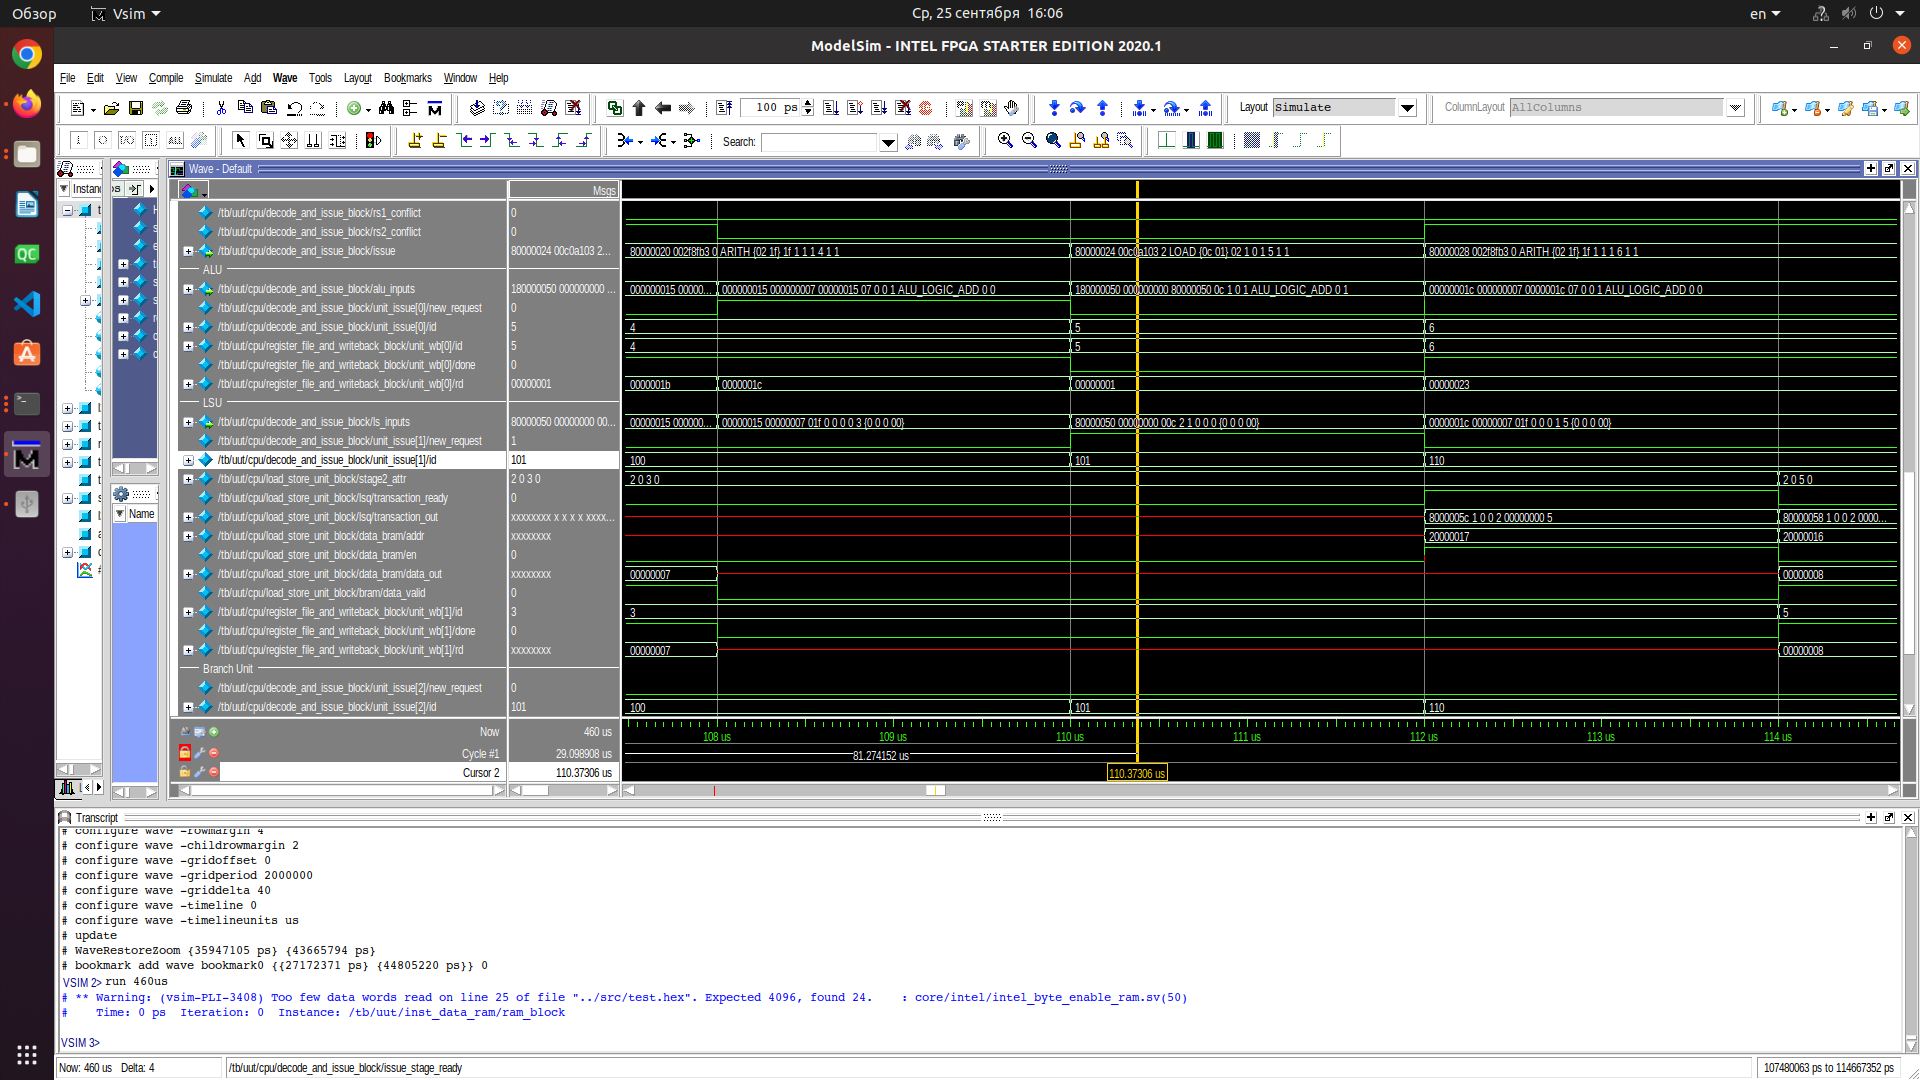
\includegraphics[width=0.9\textwidth]{runstart}
	\caption{1-й такт стадии выполнения для 2-й итерации 80000024}
	\label{fig:runstart}
\end{figure}

\begin{figure}[h]
	\centering
	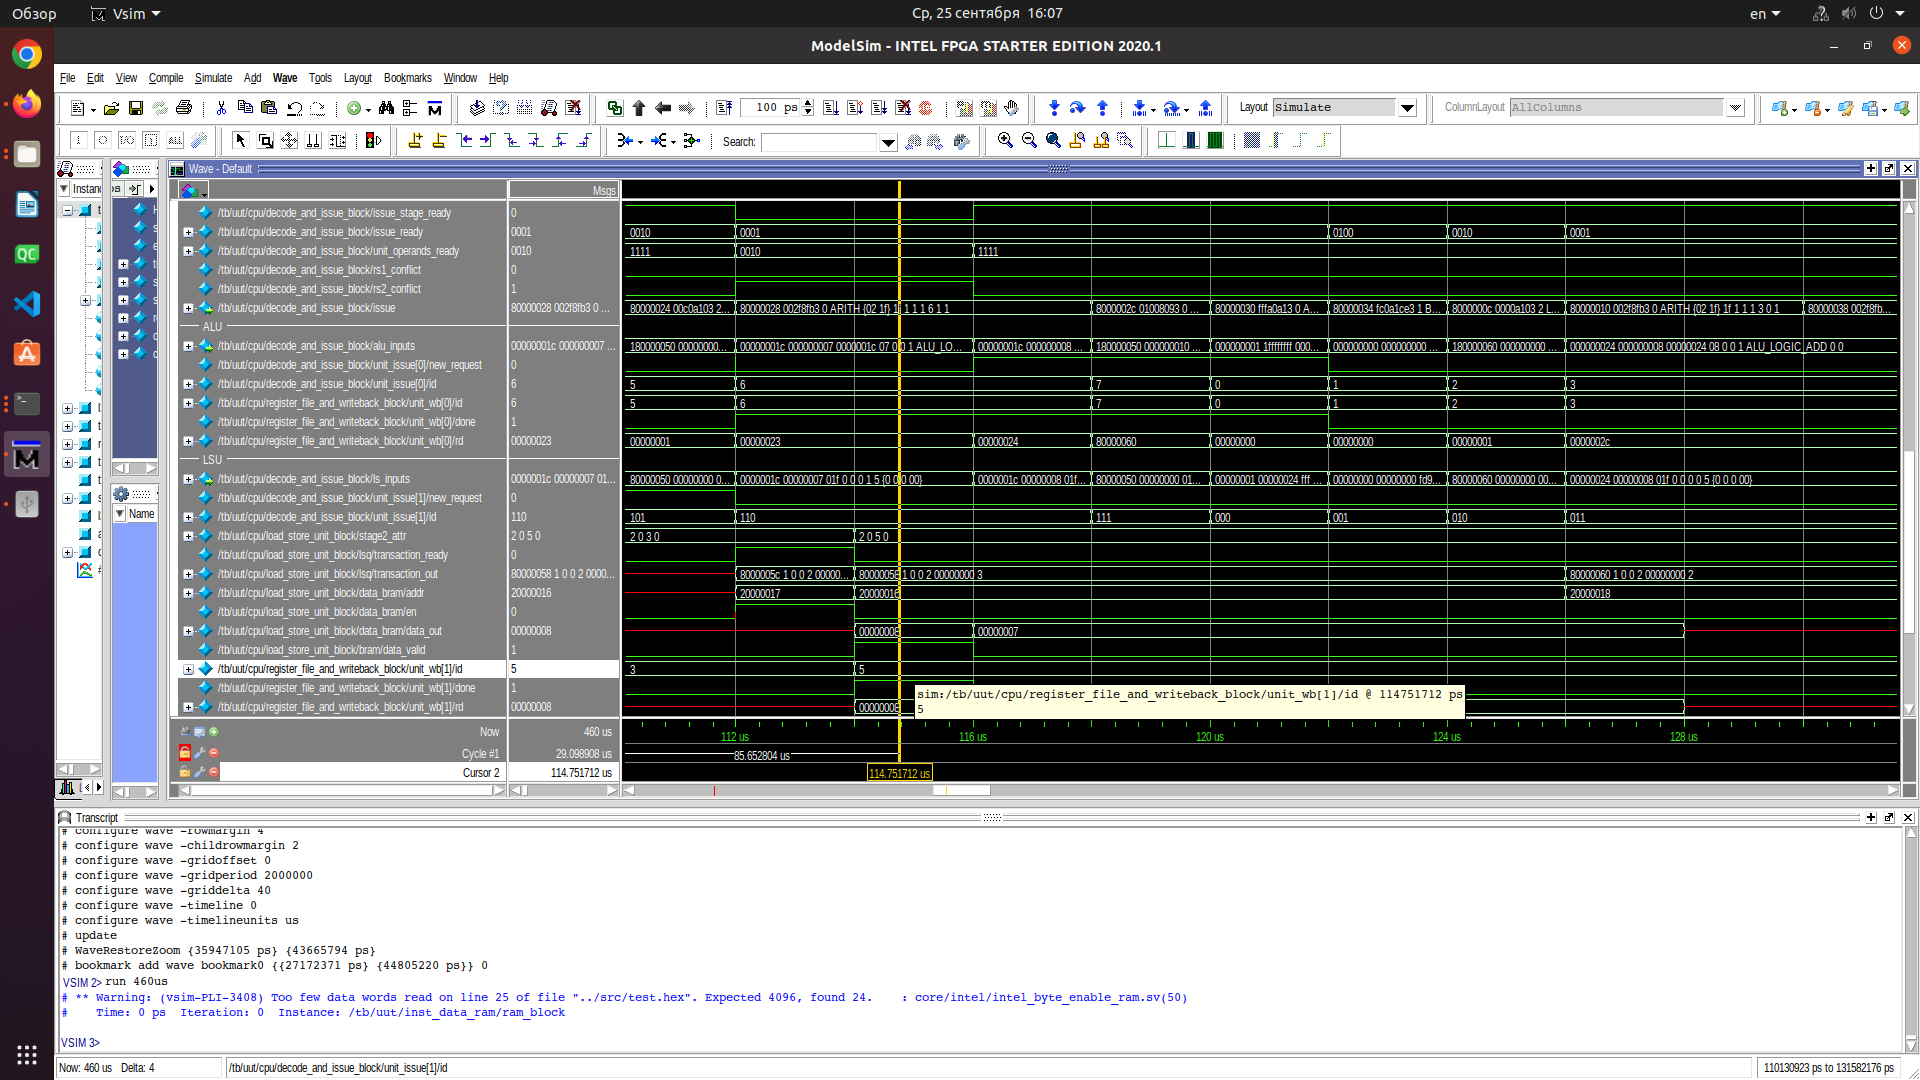
\includegraphics[width=0.9\textwidth]{runend}
	\caption{3-й такт стадии выполнения для 2-й итерации 80000024}
	\label{fig:runend}
\end{figure}

\clearpage

\section{Задание №5}

\begin{figure}[h]
	\centering
	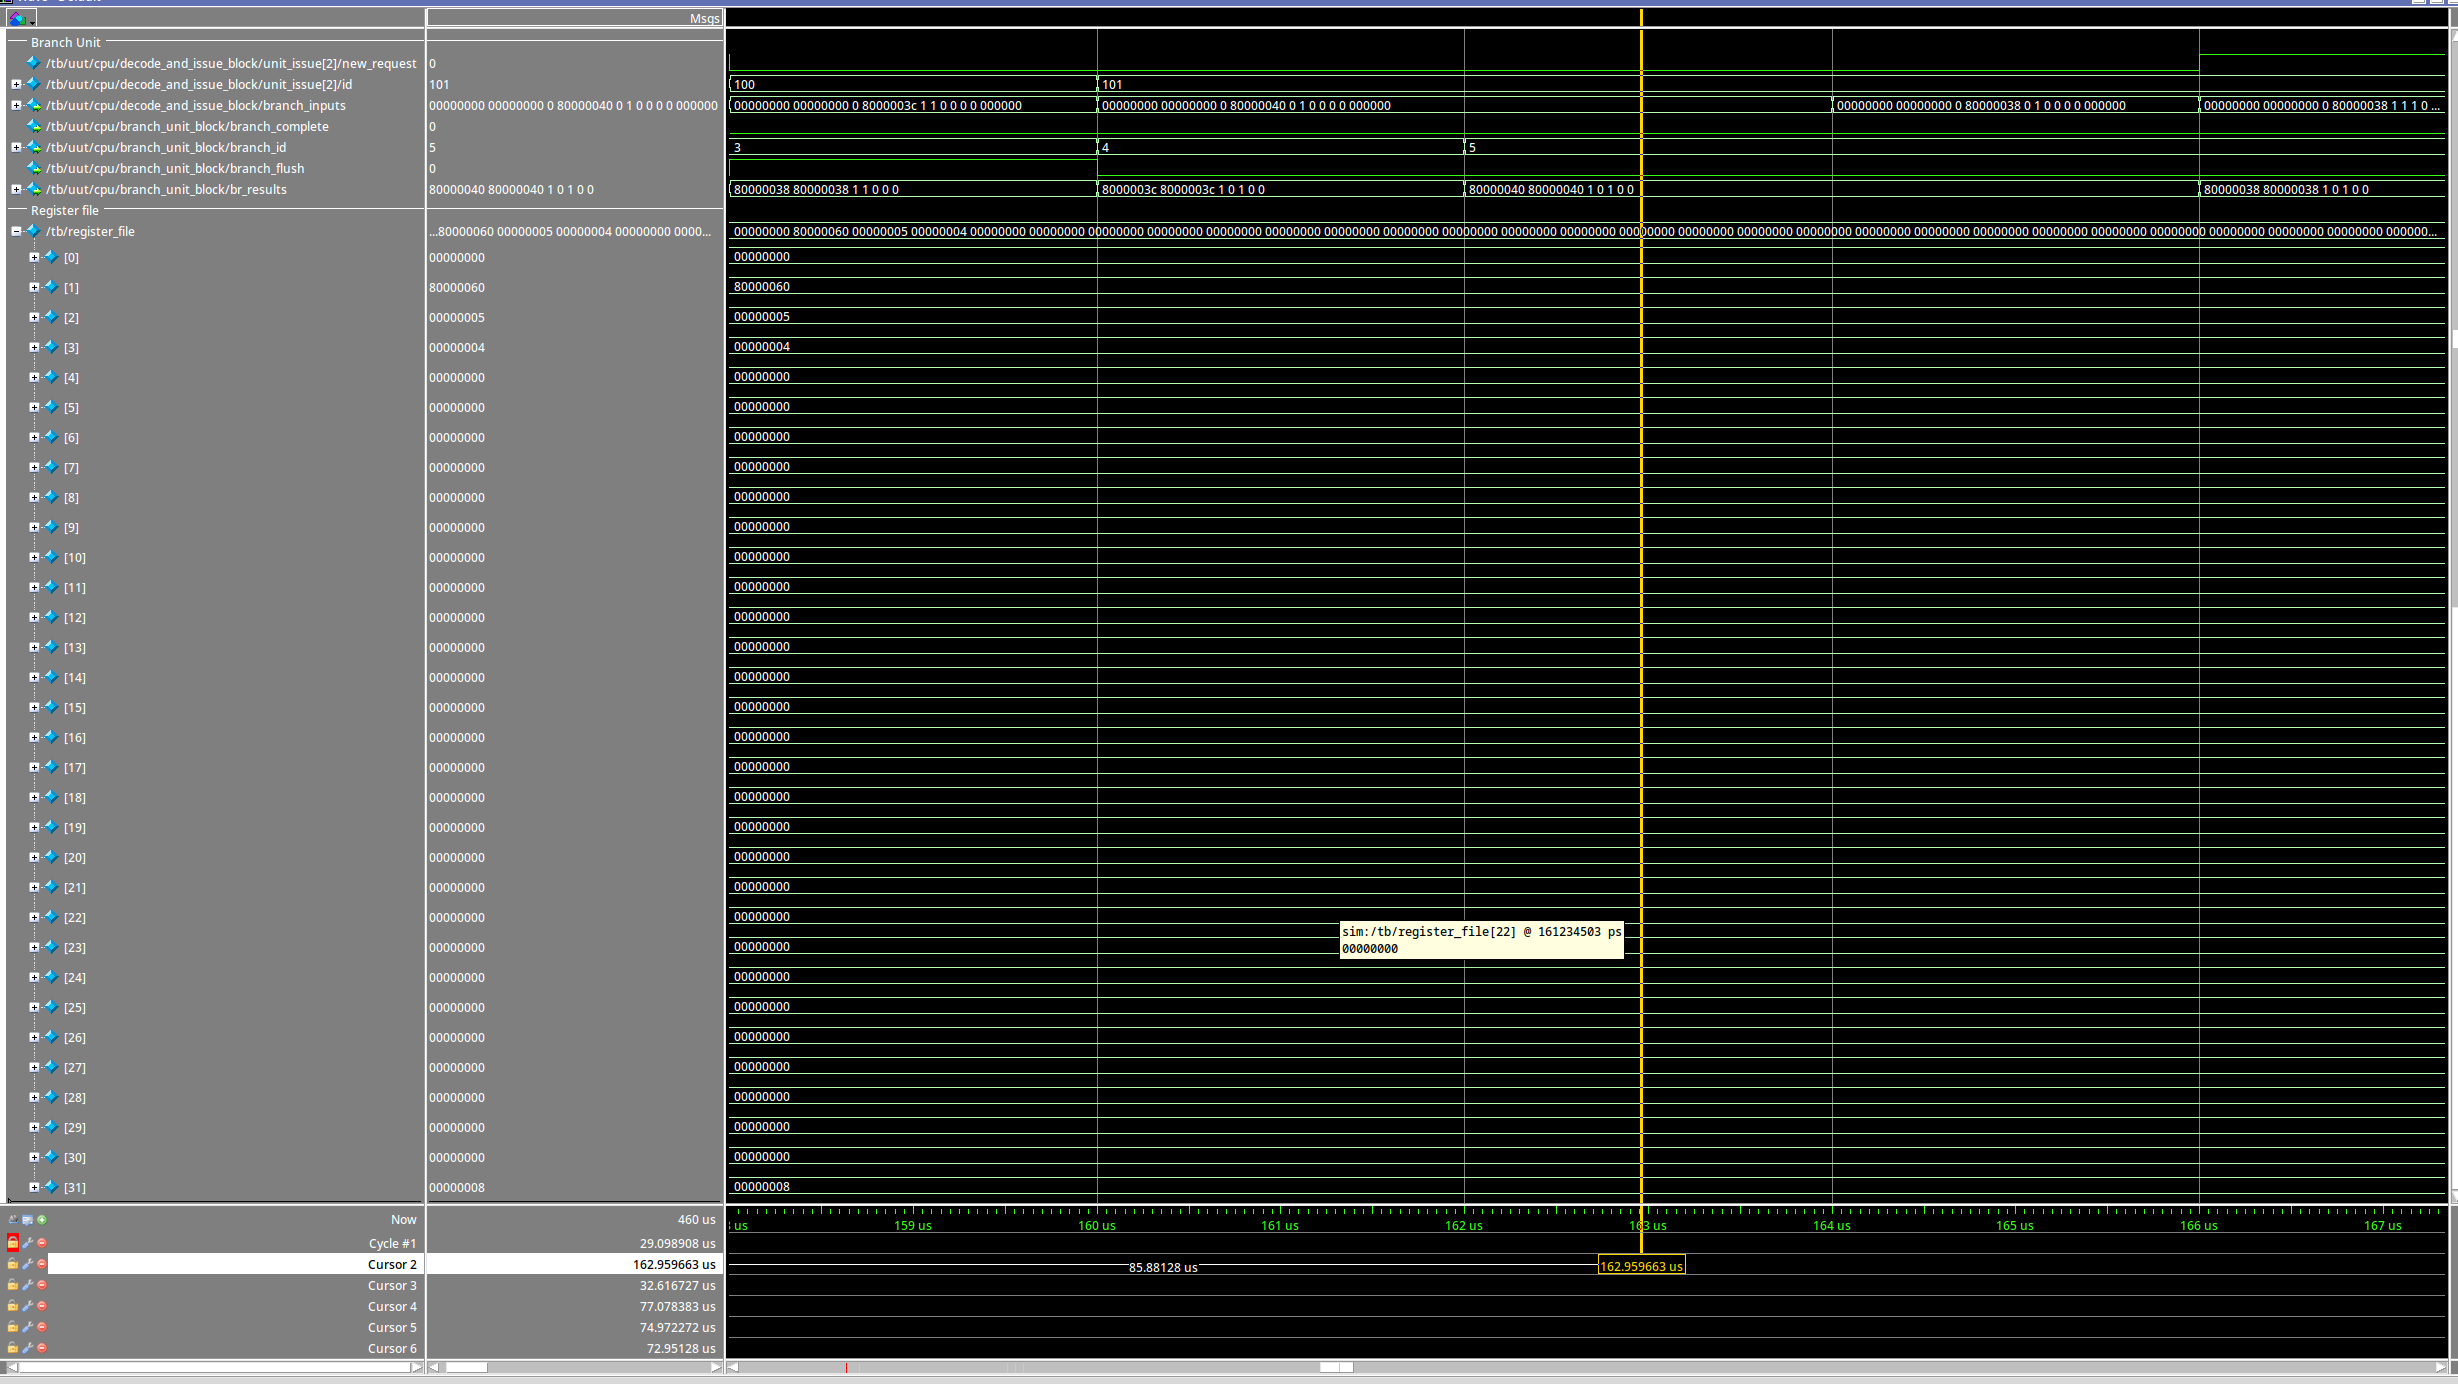
\includegraphics[width=0.9\textwidth]{endx31}
	\caption{Значение регистров после окончания работы программы}
	\label{fig:endx31}
\end{figure}

На рисунке (\ref{fig:endx31}) можно увидеть, что значение регистра x31 на момент окончания программы равно 8, как и было предсказано в задании 1.

\begin{figure}[h]
	\centering
	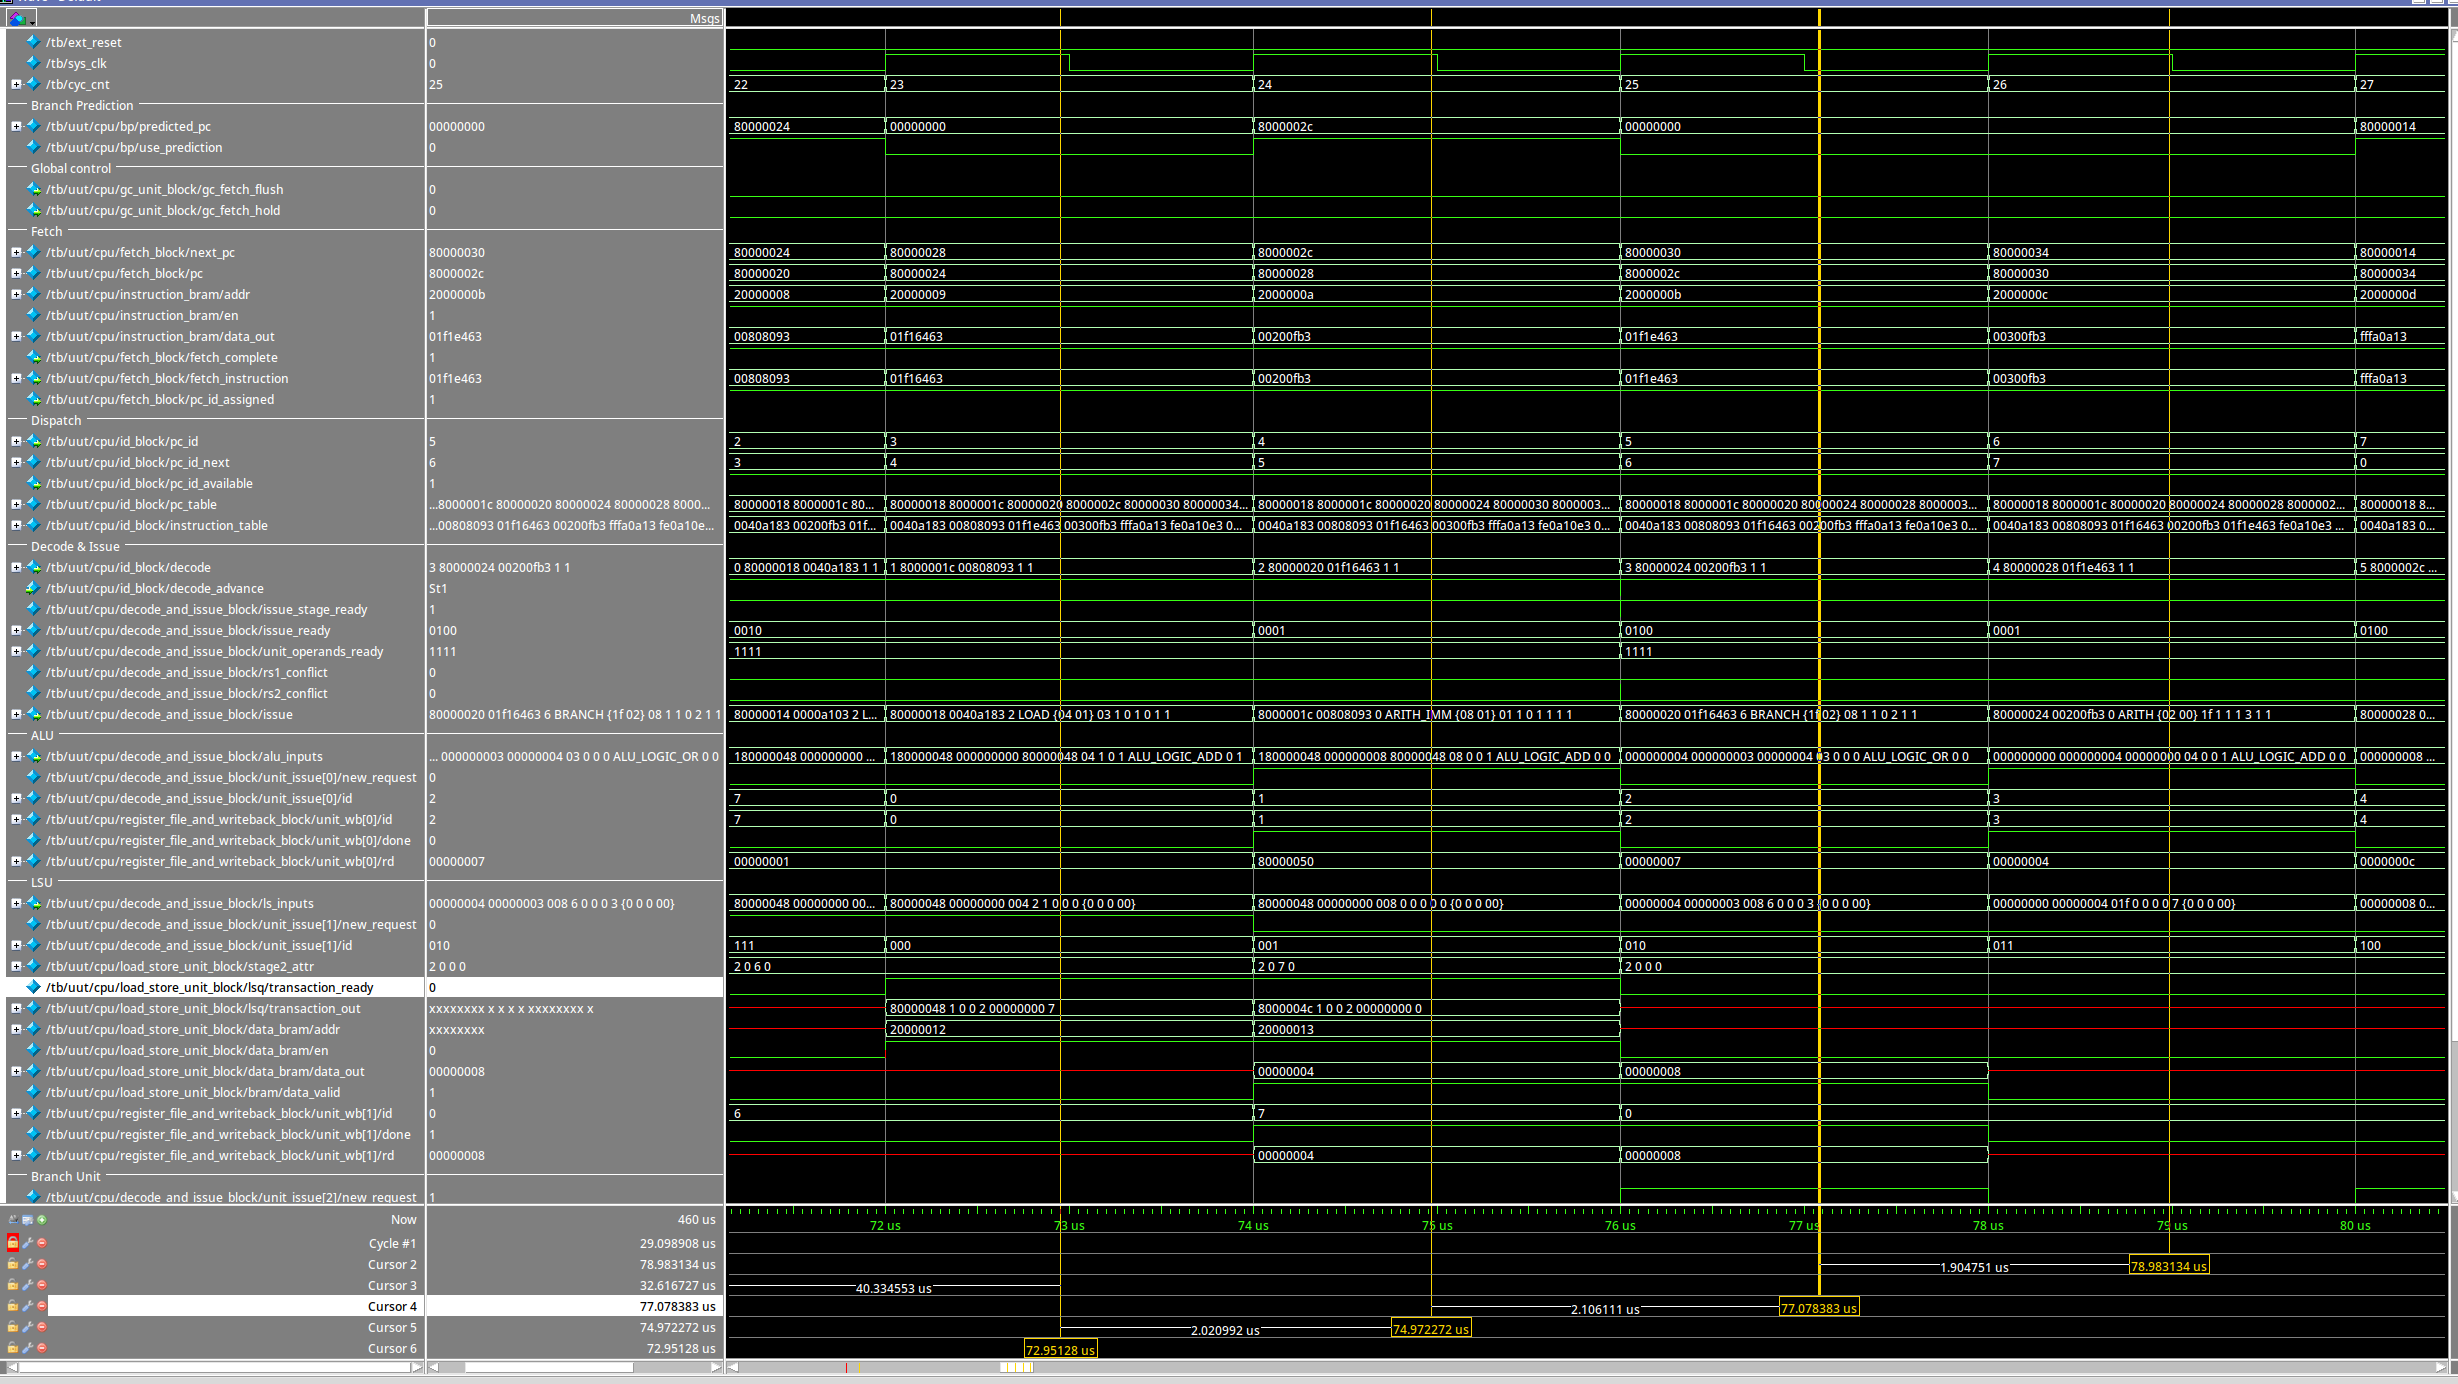
\includegraphics[width=0.9\textwidth]{testpom}
	\caption{Трасса команды отмеченной \#! в листинге \ref{test}}
	\label{fig:testpom}
\end{figure}

На рисунке (\ref{fig:testpom}) представлены все стадии команды отмеченной \#! в листинге \ref{test}.

\begin{figure}[h]
	\centering
	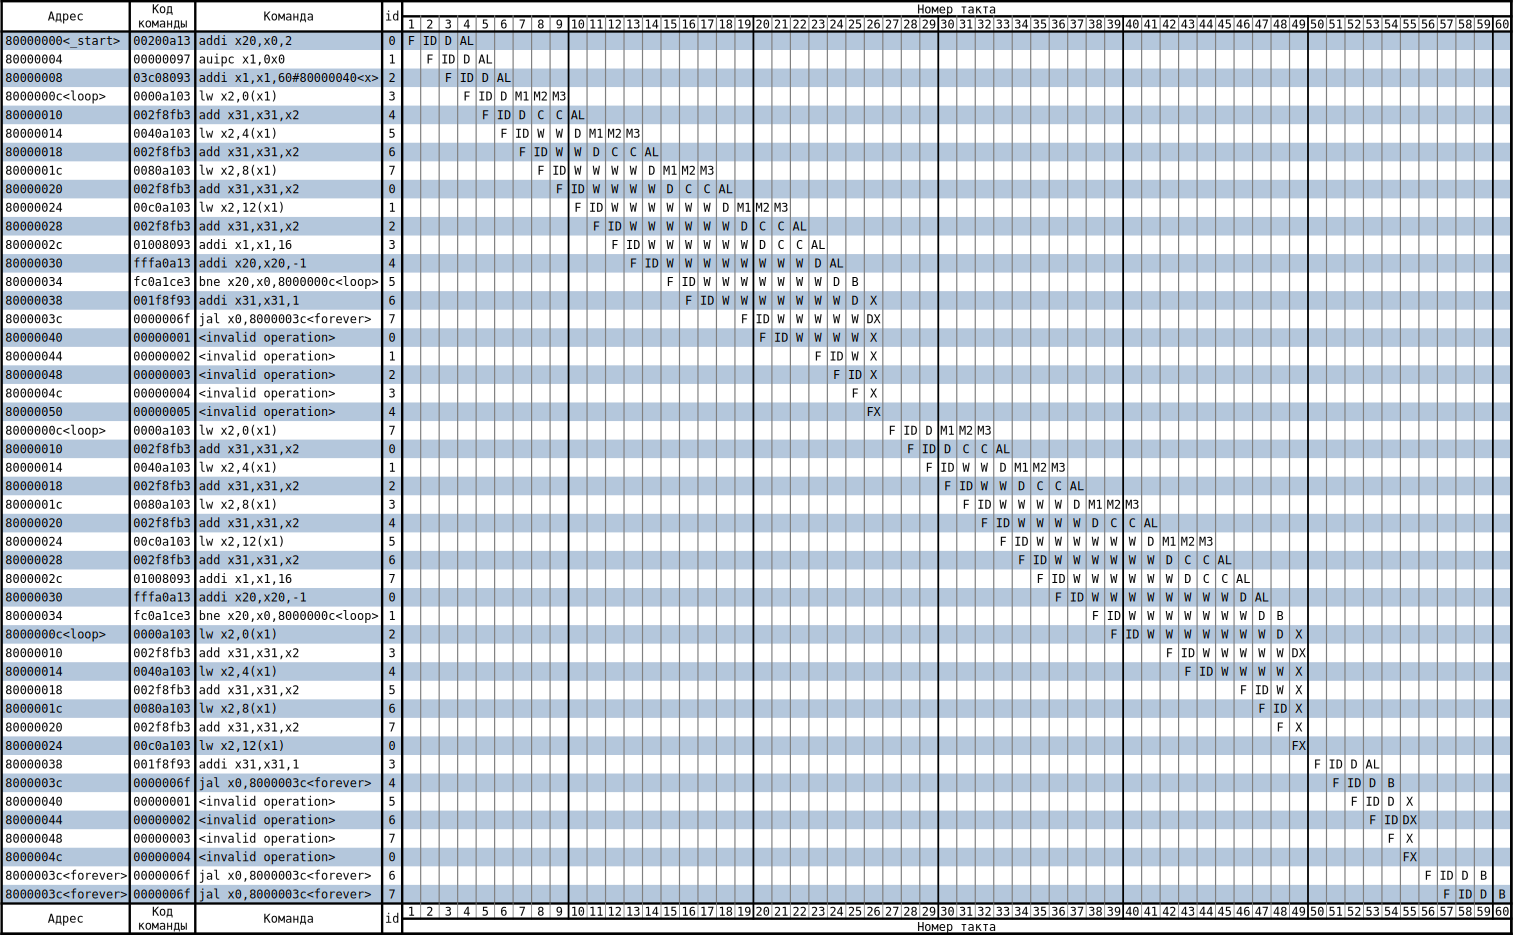
\includegraphics[width=0.9\textwidth]{pipeline}
	\caption{Трасса программы в листинге \ref{test}}
	\label{fig:pipeline}
\end{figure}

На рисунке (\ref{fig:pipeline}) представлена трасса программы по варианту. Как видно программа достаточно хорошо оптимизирована, так как в ней нет конфликтов при обращения к ресурсам, а значит и нет задержек. Единственное что можно оптимизировать - количество сбросов конвейера из-за условных переходов.

Для этого заменим поиск максимума через сравнение с условным переходом на конструкцию:

\begin{lstlisting}[label=max,caption={Поиск максимума через логические и арифметические операции.}]
	c = b - a
	k = 1 if a < b else 0
	k-- (с переполнением)
	max = b - d & c
\end{lstlisting}

Данная конструкция легко реализуется с помощью команд заданной архитектуры. Оптимизированный листинг представлен на (\ref{optimized})

\begin{lstlisting}[label=optimized,caption={Оптимизированная программа по варианту}]
  .section .text
	.globl _start;
	len = 9 #Размер массива
	enroll = 2 #Количество обрабатываемых элементов за одну итерацию
	elem_sz = 4 #Размер одного элемента массива
	
	_start:
	la x1, _x
	addi x20, x0, (len-1)/enroll
	lw x31, 0(x1)
	addi x1, x1, elem_sz*1
	lp:
	lw x2, 0(x1)
	lw x3, 4(x1)
	add x1, x1, elem_sz*enroll
	
	sub x4, x31, x2
	slt x5, x2, x31 # x5 = 1 if x2 < x31
	addi x5, x5, -1 # x5 = 11.....11 if x2 > x31
	and x4, x4, x5  # x4 = 0 if x2 < x31
	sub x31, x31, x4
	
	sub x4, x31, x3
	slt x5, x3, x31 # x5 = 1 if x3 < x31
	addi x5, x5, -1 # x5 = 11.....11 if x3 > x31
	and x4, x4, x5  # x4 = 0 if x3 < x31
	sub x31, x31, x4
	
	addi x20, x20, -1
	bne x20, x0, lp
	lp2: j lp2
	
	.section .data
	_x:     .4byte 0x1
	.4byte 0x2
	.4byte 0x3
	.4byte 0x4
	.4byte 0x8
	.4byte 0x6
	.4byte 0x7
	.4byte 0x5
	.4byte 0x4
\end{lstlisting}

Трасса оптимизированной программы на рисунке (\ref{optimized_pipeline})

\begin{figure}[h]
	\centering
	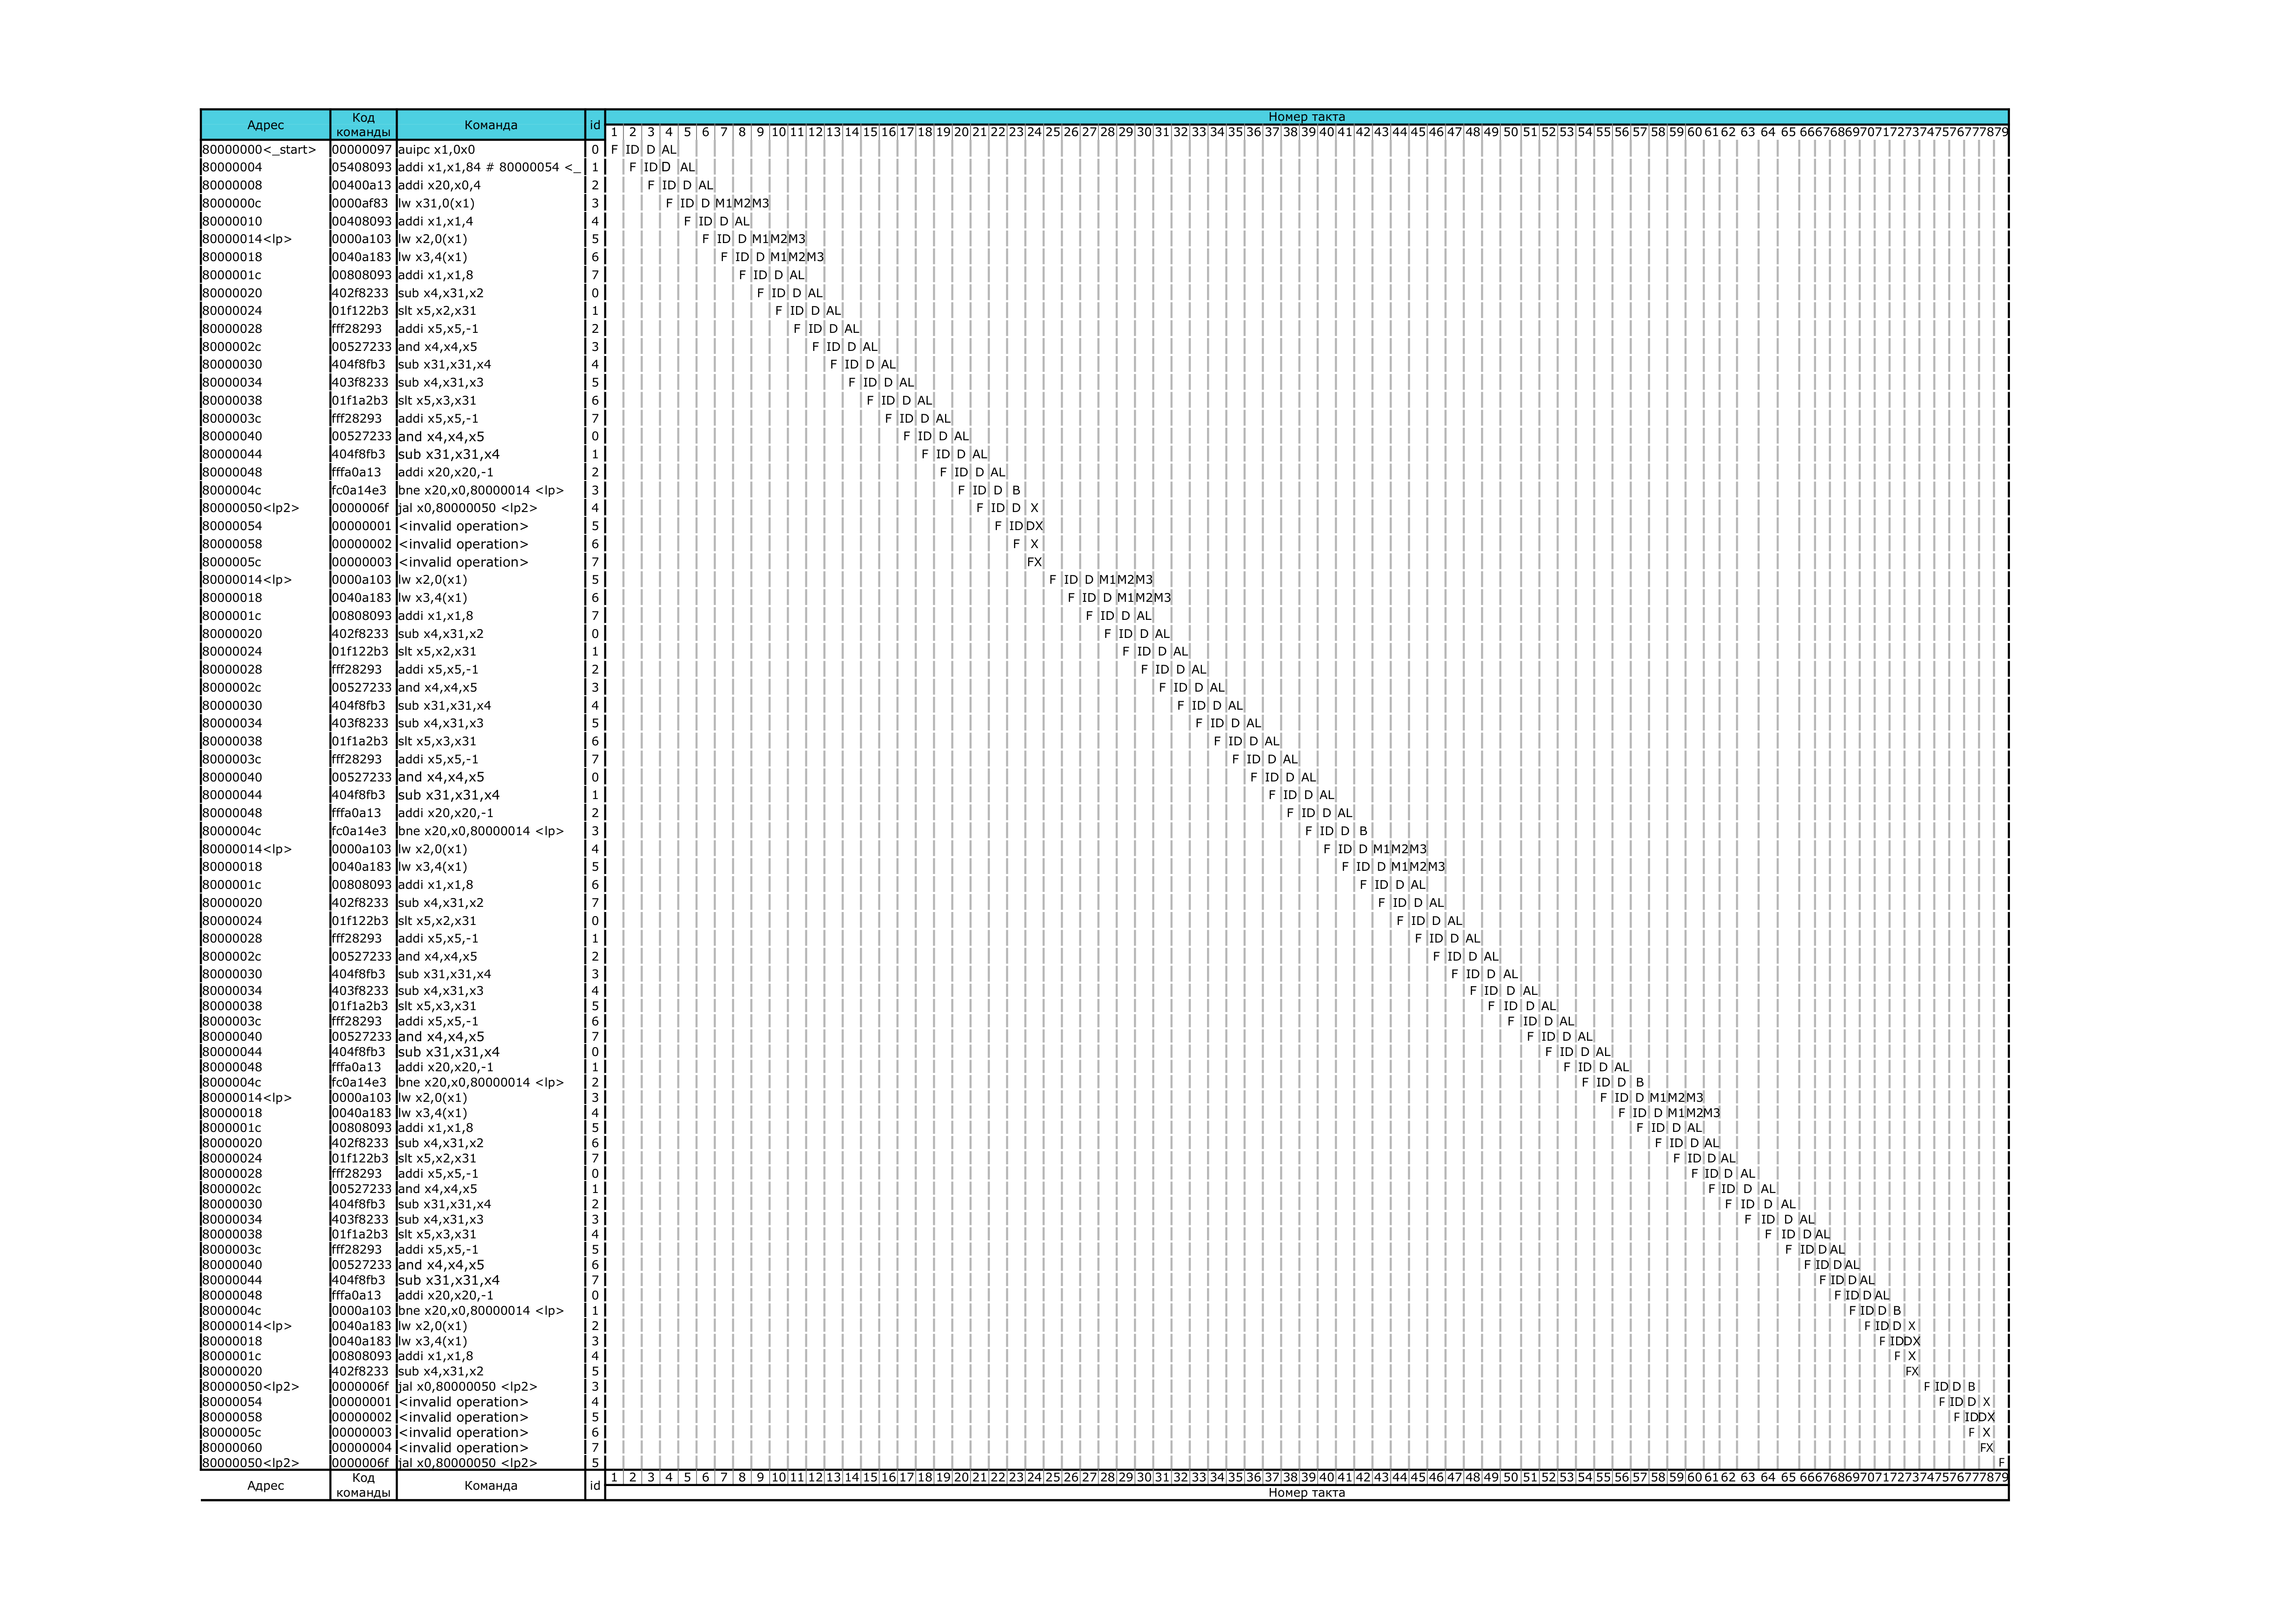
\includegraphics[width=\textwidth]{pipeline_optimized}
	\caption{Трасса оптимизированной программы в листинге \ref{optimized}}
	\label{fig:optimized_pipeline}
\end{figure}

Как видно в программе стало меньше сбросов конвейера, тем не менее количество тактов стало больше(79 и 67), так как поиск максимума без условий требует больше команд. Однако в другой конфигурации массива, где блок предсказателя чаще ошибался, возможно оптимизированная программа была бы эффективная.

\clearpage
